\chapter{Vorgehensweise}\label{chap:Vorgehensweise}
Um dem im Kapitel \glqq{}\ref{chap:Motivation} Motivation\grqq{} formulierten Ziel zu folgen, muss zunächst eine Datenquelle gewählt werden.
Anschließend werden deren Daten in eine nutzbare Form übertragen.
Schlussendlich können die Informationen aus den Daten verknüpft, interpretiert und graphisch dargestellt werden.

Der mit Jupyter Notebook (\href{jupyter.org}{jupyter.org}) erstellte Programmcode findet sich in den Programmdateien im Anhang der Bachelorarbeit.

Diese Bachelorarbeit basiert teilweise auf den Vorleistungen des Bachelorprojekts zur Visualisierung der COVID-19-Daten von Leander Marius Bürkin.
Ziel dieses Bachelorprojekts war eine Reihe an Deutschlandkarten in einem Video zusammenzufassen, welches die Ausbreitung der COVID-19-Pandemie in Deutschland vom ersten März 2020 bis zum letzten Tag, für den die API des Robert Koch-Instituts Daten liefert, darstellt.


Das Bachelorprojekt sowie eines der Videos ist verfügbar unter\\
\href{https://github.com/leanderbuerkin/Bachelorprojekt/blob/master/media/germany_incidence_V4_300ms_1080p_music.mp4}{https://github.com/leanderbuerkin/Bachelorprojekt/blob/master/media/}\\
\href{https://github.com/leanderbuerkin/Bachelorprojekt/blob/master/media/germany_incidence_V4_300ms_1080p_music.mp4}{germany\_incidence\_V4\_300ms\_1080p\_music.mp4}

\section{Datenquellen - Ursprung und Abspeicherung}\label{sec:Datenquelle}

Das gannnte Bachelorprojekt sowie diese Bachelorarbeit verwenden Informationen zur COVID-19-Pandemie und den geographischen Daten von 412 deutschen Landkreisen. Alle Daten stammen von der Programmierschnittstelle (API) des Robert Koch-Instituts \glqq{}COVID-19 Datenhub\grqq{}
(\href{npgeo-corona-npgeo-de.hub.arcgis.com}{npgeo-corona-npgeo-de.hub.arcgis.com}) oder werden aus den daher stammenden Daten generiert. Diese Datenquelle wurde gewählt, weil sie vom Robert Koch-Institut (RKI, \href{www.rki.de}{www.rki.de}) und dem deutschen Staat\\
 (www.bundesregierung.de) referenziert wird. Beispielsweise unter:
\begin{itemize}
    \item \href{www.bundesregierung.de/breg-de/themen/coronavirus}{www.bundesregierung.de/breg-de/themen/coronavirus}
    \item \href{www.rki.de/DE/Content/InfAZ/N/Neuartiges_Coronavirus/Daten/Fallzahlen_Inzidenz_aktualisiert.html}{www.rki.de/DE/Content/InfAZ/N/Neuartiges\_Coronavirus/Daten/Fallzahlen}\\
    \href{www.rki.de/DE/Content/InfAZ/N/Neuartiges_Coronavirus/Daten/Fallzahlen_Inzidenz_aktualisiert.html}{\_Inzidenz\_aktualisiert.html}
\end{itemize}

Insgesamt werden drei verschiedene Datenpakete der API verwendet, zum einen die geographischen Daten der Landkreise, zum anderen die Summe aller aufgetretenen COVID-19-Fälle seit Beginn der Pandemie für jeden Landkreis und jeden Tag vom 01.03.2020 bis zum 21.07.2021 sowie eine Auflistung aller Meldungen der Gesundheitsämter, in welchen das  Referenzdatum, das Meldedatum, die Anzahl der betroffenen Menschen und deren Zustand (entweder genesen, verstorben oder noch infektiös) angegeben werden. Das Referenzdatum kann laut RKI als Tag der Infektion interpretiert werden, das Meldedatum als Genesungsdatum beziehungsweise Sterbedatum \autocite{RKI_Bulletin}.

Alle drei Datenpakete liefern Daten für die deutschen Landkreise. Diese sind jeweils in Form des sogenannten Gemeindeschlüssels referenziert, eine vollständige Zuordnung der Landkreise sindet sich in \autoref{tab:counties_by_admunitid}. Die Gemeindeschlüssel bestehen aus vier oder fünf Ziffern, wobei die erste oder die ersten beiden das Bundesland angeben, die zweite bzw. dritte Stelle gegebenenfalls den Regierungsbezirk und die letzten beiden Stellen bestimmen den Landkreis. Somit lassen sich die Landkreise in Regierungsbezirke einteilen und mithilfe der Kennzahlen der Landkreise die Kennzahlen der Regierungsbezirke berechnen.

Die Landkreise, welche das RKI angibt, stimmen nicht mit den Landkreisen des Statistischen Bundesamtes  \autocite{statistischesBundesamtLandkreise}
überein: In den Daten des RKIs gibt es 118 Landkreise mehr, beziehungsweise wenn man die kreisfreien Städte abzieht, zwölf Landkreise mehr. Diese Diskrepanz kommt durch die Aufteilung von Berlin in seine 12 Bezirke. Zudem wird Eisenach in den Daten des RKIs als eigene kreisfreie Stadt gewertet und nicht zum Wartburgkreis hinzugezählt. Der Stadtkreis Eisenach ist mit dem Gemeindeschlüssel 16056 versehen. Trotz dieser Unterschiede und obwohl auch kreisfreie Städte miteinbegriffen sind, wird im folgenden weiterhin der Begriff \glqq{}Landkreise\grqq{} für alle 412 Gebiete verwendet.

Der Gemeinde
%Liste der NUTS-Codes Gemeindeschlüssel leiten sich daraus ab. URL siehe Kommentar
%https://eur-lex.europa.eu/legal-content/DE/TXT/PDF/?uri=CELEX:32016R2066&from=EN
Die Regierungsbezirke, welche sich aus den ersten zwei oder drei Stellen des Gemeindeschlüssels ergeben, stimmen leider auch nicht mit den Regierungsbezirken des Statistischen Bundesamtes
\autocite{statistischesBundesamtRegierungsbezirke}
überein: Die Gemeindeschlüssel haben 38 verschiedene Präfixe, wohingegen laut statistischem Bundesamt aktuell nur 19 Regierungsbezirke existieren.
Da jedoch nicht alle Bundesländer in Regierungsbezirke unterteilt sind, wird in neun Fällen das Bundesland an Stelle möglicher Regierungsbezirke verwendet. Die Diskrepanz von neun weiteren Gebieten entsteht durch die Veränderung der Regierungsbezirke seit der Einführung der Gemeindeschlüssel: Die Gemeindeschlüssel Niedersachsens lassen auf 4 Regierungsbezirke schließen, die Gemeindeschlüssel der Rheinland-Pfalz auf 3 und die Gemeindeschlüssel Sachsens auf 3 weitere. Keines dieser Bundesländer ist aktuell noch in Regierungsbezirke unterteilt. Somit ergeben sich 19 echte Regierungsbezirke, 10 ehemalige sowie 9 Bundesländer ohne Regierungsbezirke.
Trotz dieser Unterschiede und obwohl auch Bundesländer miteinbegriffen sind, wird im folgenden weiterhin der Begriff \glqq{}Regierungsbezirk\grqq{} für alle 38 Gebiete verwendet.

Die genannten Daten werden abgespeichert, damit sie nicht bei jeder Ausführung erneut angefordert und aufbereitet werden müssen.
\section{Datenaufbereitung}
Bevor die Daten genutzt werden können, müssen sie verifiziert werden, überflüssige Informationen entfernt werden und neue Kennzahlen aus den gegebenen Informationen berechnet werden. Daten vor der Datenaufbereitung, welche direkt von der API oder einem Backup davon stammen, werden als \glqq{}unmodifizierte\grqq{} Daten bezeichnet. 

Daten, die rudimentär auf Vollständigkeit überprüft wurden, aus den Daten generierte Daten enthalten und bei welchen überflüssige Informationen entfernt wurden, werden \glqq{}modifizierte\grqq{} Daten genannt.

Zunächst werden die unmodifizierten Daten in eine übersichtlichere Form übertragen und es wird sichergestellt, dass gleich viele Werte für jeden Landkreis vorhanden sind. Zudem werden die Umrisse der 100 Landkreise von Hand geprüft, welche mehrere Polygone enthalten, diese werden entweder als Ausschnitt oder als reale Fläche interpretiert. Würde man einfach alle Polygone zeichnen, kann es passieren, das ein Bereich, welcher komplett von einem Landkreis umgeben ist von einem seiner Polygone übermalt wird, welches genau diese Fläche aus dem Landkreis ausschneiden sollte.

Nachdem die unmodifizierten Daten in eine übersichtlichere Form übertragen und überprüft wurden, werden aus den Daten weitere Werte berechnet.

Die Bevölkerungsdichte der Landkreise wird berechnet, indem die Anzahl der Einwohner durch die Fläche in Quadratmetern geteilt wird (siehe \autoref{eq:Bevölkerungsdichte}). Beide Informationen werden von der API bereitgestellt.
Die Bevölkerungsdichte wird auch für die Regierungsbezirke berechnet. 
Sowohl die Bevölkerungsdichten der Landkreise wie auch die Bevölkerungsdichten der Regierungsbezirke werden zur Einordnung der Korrelationsanalysen auf einer Deutschlandkarte dargestellt, wobei die Farbe die Bevölkerunsdichte repräsentiert, wie in \autoref{sec:Grundlagen:Farbgebung} beschrieben.

Für jeden Landkreis und jeden Regierungsbezirk wird eine Zeitreihe mit den 7-Tage-Inzidenzen angefertigt, welche die 7-Tage-Inzidenz nach \autoref{eq:7-Tages_Inzidenz} für jeden Tag enthält, für den eine Fallzahlen angegeben ist. 

Um die Auflistung aller Meldungen der Gesundheitsämter nutzen zu können, müssen diese erst für jeden Landkreis und jeden Tag gesammelt und aufsummiert werden:
Das Referenzdatum wird als Tag der Infektion interpretiert. Die Anzahl der betroffenen Individuen wird für jeden folgenden Tag zur akkumulierten Anzahl der Fälle hinzuaddiert.
Das Meldedatum wird als Tag der Genesung beziehungsweise Tag des Todes interpretiert, je nachdem ob die Meldung Genesung oder Tod angibt. Die Anzahl der betroffenen Individuen wird hier zum einen für jeden folgenden Tag zur akkumulierten Anzahl der Genesenen/Verstorbenen hinzuaddiert. Zum anderen wird die Anzahl der betroffenen Individuen für jeden Tag zwischen dem Referenzdatum und dem Meldedatum zu den aktiven Fällen hinzuaddiert.

Mithilfe der Gesamtbevölkerung eines Landkreises werden aus diesen Daten für jeden Tag und jeden Landkreis alle drei Kategorien des SIR-Modells berechnet:

\begin{itemize}
    \item \glqq{}susceptible\grqq{}: Die Gesamtbevölkerung des Landkreises minus die akkumulierte Anzahl der Fälle.
    \item \glqq{}infectious\grqq{}: Liegt als aktive Fälle bereits vor.
    \item \glqq{}recovered\grqq{}:
    Die Summe aus der akkumulierten Anzahl der Genesenen und der Verstorbenen. Oder die akkumulierte Anzahl der Fälle minus die aktiven Fälle. Solange zu jeder Meldung ein Referenzdatum angegeben ist, entspricht das Ergebniss der zweiten Berechnungsvariante dem der ersten.
\end{itemize}

Um ein Gefühl dafür zu bekommen, welcher Lankreis in welchem Ausmaß von der COVID-19-Pandemie getroffen wurde, wird die akkumulierte Anzahl der COVID-19-Fälle des letzten Tages durch die Bevölkerung des Landkreises geteilt und farblich in einer Deutschlandkarte dargestellt.
%
\section{Datenformat}\todo{Muss entweder noch umgeschrieben werden, wodurch es sehr lang wird oder massiv gekürzt werden. Ich warte noch auf Antwort von meinem Betreuer, Korrekturleser können bei 3.4 Datendarstellung weitermachen}
Die Daten liegen in einer Kombination aus sogenannten Python Dictionaries und sogenannten Python Listen vor.

Ein Dictionary ist dadurch charakterisiert, dass man über den Namen eines Elements (\glqq{}Key\grqq{}) das Element (\glqq{}Value\grqq{}) bekommt, ähnlich wie man früher in Telefonbüchern anhand des Namens (Key) die Telefonnummer (Value) erhalten hat.

Listen sind dadurch charakterisiert, dass sie Elemente in einer fixen Reihenfolge enthalten und sich diese durch ihren Index leicht auffindbar machen. So sind beispielsweise die Anzahl der COVID-19-Fälle der einzelnen Tage chronologisch in einer Liste gespeichert, sodass man daraus direkt eine Abbildung erstellen kann.


Die Programmdateien erstellen drei verschiedene sogenannte globale Dictionaries, welche (in untergeordneten Dictionaries und Listen) alle Daten enthalten. Globale Dictionaries sind in allen Dateien verfügbar und unterscheiden sich insofern von lokalen Dictionaries/Listen, welche nur in einzelnen Programmabschnitten vorliegen und daher nicht derart zentral sind.
Die drei Dictionaries heißen
\begin{itemize}
    \item covid19
    \item counties\_geography
    \item non\_county\_specific\_data
    \item districts
\end{itemize}

\textbf{covid19}\\
Das Dictionary covid19 speichert die COVID-19-Fälle jedes deutschen Landkreises und die daraus berechnete sieben Tages Inzidenz sowie die um den Mittelwert der 7-Tage-Inzidenzen verminderten Inzidenzen.

Mit dem Gemeindeschlüssel eines Landkreises als Key und dem zusätzlichen Key \glqq{}cases\grqq{} erhält man die akkumulierte Anzahl an COVID-19-Fällen pro Tag des Landkreises als Liste.

Mit dem Gemeindeschlüssel eines Landkreises als Key und dem Key \glqq{}incidences\grqq{} erhält man die sieben Tages Inzidenz pro Tag des Landkreises als Liste.

Mit dem Gemeindeschlüssel eines Landkreises als Key und dem Key \glqq{}incidences\_scaled\grqq{} erhält man die sieben Tages Inzidenz pro Tag des Landkreises als Liste.

Alle drei Listen enthalten für jeden Tag seit dem 01.03.2020 bis zu dem Tag der aktuellsten Daten jeweils einen Eintrag.

Die Anzahl an COVID-19-Fällen pro Tag stammt aus dem \glqq{}COVID-19 Datenhub\grqq{}. Die sieben Tages Inzidenz wird wie in \autoref{sec:Grundlagen:7-Tage-Inzidenz} beschrieben aus den Daten vom COVID-19 Datenhub berechnet.

\todo{Aufbau des Gemeindeschlüssels erklären}
\textbf{counties\_geography}\\
Das Dictionary counties\_geography enthält zu jedem Landkreis ein Dictionary mit den folgenden Elemente:
\begin{itemize}
    \item[name:] Der Name des Landkreises
    \item[population:] Die Einwohnerzahl des Landkreis aus einer offiziellen Schätzung (nähere Informationen finden sich im COVID-19 Datenhub). Diese Zahlen werden auch für die offizielle Berechnung der sieben Tages Inzidenz verwendet.
    \item[area\_in\_m2:] Die Fläche des Landkreises in Quadratmetern
    \item[geometry:] Die Form des Landkreises in einer für die Darstellung angepassten Form
    \item[raw\_geometry:] Die Form des Landkreises in der originalen Form
    \item[population\_density:] Die Bevölkerungsdichte des Landkreises, berechnet aus der Fläche des Landkreises und seiner Einwohnerzahl
\end{itemize}
Außer die Bevölkerungsdichte, welche berechnet wird, und die angepassten Formen der Landkreise, welche aus den origialen Formen generiert werden, stammen alle Daten direkt aus dem \glqq{}COVID-19 Datenhub\grqq{}.

\textbf{non\_county\_specific\_data}
Das Dictionary non\_county\_specific\_data enthält die folgenden Elemente:
\begin{itemize}
    \item[unixtime:] Die Unixzeit, wie sie vom COVID-19 Datenhub zur Verfügung gestellt wird: Die Zahl der Millisekunden seit dem 01.01.1970 00:00 Uhr UTC. Die Zahl der COVID-19-Fälle und die sieben Tages Inzidenz eines entsprechenden Tages befinden sich an der selben Stelle in Ihrer jeweiligen Liste, wie der Tag in dieser Liste.
    \item[states:] Die Name und Nummern der deutschen Bundesländer. Die ersten beiden oder die erste Zahl des Gemeindeschlüssel eines Landkreises geben das Bundesland an, in welchem der Landkreis liegt. Die ersten zwei bzw. drei Zahlen geben den Regierungsbezirk an, in dem der Landkreis. Sollte es im jeweiligen Bundesland keine Regierungsbezirke geben, entspricht dies dem Bundesland.
    \item[highest\_case\_number:] Die höchste akkumulierte Fallzahl unter allen Landkreisen.
    \item[lowest\_case\_number:] Die niedrigste akkumulierte Fallzahl unter allen Landkreisen.
    \item[highest\_incidence:] Die höchste sieben Tages Inzidenz eines Tages unter allen Landkreisen.
    \item[lowest\_incidence:] Die niedrigste sieben Tages Inzidenz eines Tages unter allen Landkreisen.
    \item[UTC:] Die Unixzeit konvertiert in die Koordinierte Weltzeit im Format \glqq{}DD.MM.YYYY\grqq{}.
    \item[UTC+7days:] Die Liste der Zeiten gespeichert in UTC plus sieben weitere Tage vor dem erstem Datum in der Liste. Diese werden benutzt, um den Zeitraum der 7-Tage-Inzidenz der ersten sieben Tage darstellen zu können: die hierfür verwendeten Zeiträume beginnen jeweils vor dem ersten hier dokumentierten Fall.
\end{itemize}
\todo{itemize reparieren}
Die Unixzeit, die Namen und die Nummern der Bundesländer stammen aus dem \glqq{}COVID-19 Datenhub\grqq{}. Alle anderen Informationen wurden gesammelt oder berechnet.

In Abbildung \ref{fig:dicts_als_code} sind die drei Dictionaries dargestellt, wie sie auch im Programm verwendet werden.
\begin{figure}[H]
    \centering
    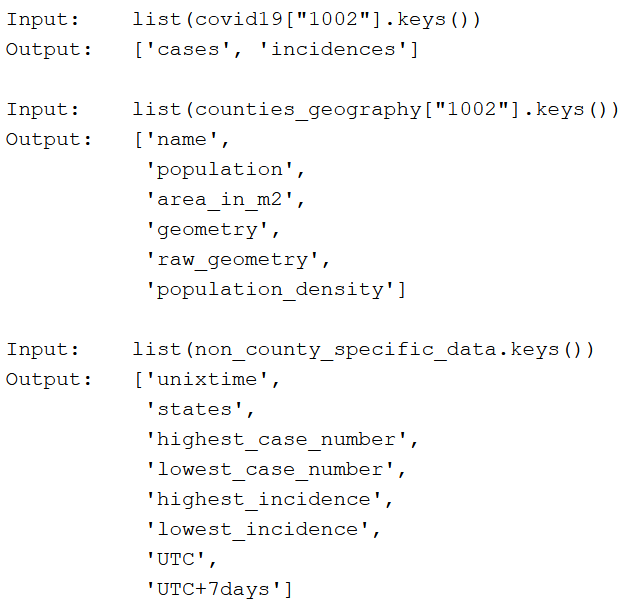
\includegraphics[width=0.8\textwidth]{figures/Vorgehensweise/Dictionarys Bachelorprojekt.png}
    \caption{
    Die Dictionaries non\_county\_specific\_data, counties\_geography und covid19 mit ihren jeweiligen Schlüsseln.
    Für die Dictionaries covid19 und counties\_geography wurde jeweils der Landkreis Kiel (Gemeindeschlüssel 1002) zur Veranschaulichung verwendet.}
    \label{fig:dicts_als_code}
\end{figure}

\todo{Daten aus Meldungen einpflegen}
\section{Datendarstellung}
Abschließend werden die Daten wie folgt dargestellt.
\subsection{Allgemeine Daten der Gebiete}
Zuerst werden die folgenden Daten der Landkreise und Regierungsbezirke dargestellt, welche auf einfachen Gleichungen beruhen und lediglich zur Einordnung der anderen Ergebnisse dienen:
\begin{itemize}
    \item Die Bevölkerungsdichte, um diese mit dem Infektionsverhalten in Zusammenhang setzen zu können.
    \item Die Anordnung der Gebiete, wenn man sie nach ihrem Gemeindeschlüssel sortiert - Die Sortierung erfolgt hier lexikographisch, das heißt, das die Länge des Gemeindeschlüssels keine Rolle spielt, sondern immer das erste Zeichen verglichen wird und bei Übereinstimmung das nächste verglichen wird. Dadurch ergibt sich eine einheitlichere Nord-Süd-Aufteilung als die Sortierung nach dem Betrag.
    \item Die Summe der 7-Tage-Inzidenzen als Maß dafür, wie stark ein Gebiet betroffen war.
\end{itemize}
\subsection{SIR-Modell}
Zudem wird anhand der Daten ein SIR-Modell erstellt.


Da jedoch die Zahl der aktiven Fälle sehr niedrig und dementsprechend sensibel gegenüber kleinen Anomalien sind, wird dieses nur auf Bundesebene erstellt. 
Hierfür werden die drei Kennzahlen des SIR-Modells in drei Abbildungen dargestellt.
\subsection{Korrelationsanalyse}
Für alle Korrelationsanalysen werden aus den in \autoref{sec:Grundlagen:7-Tages Inzidenz} genannten Gründen die 7-Tage-Inzidenzen nach \autoref{eq:7-Tages_Inzidenz} verwendet. Folgenden Gebiete werden nach den in \autoref{sec:BeschreibungKorrelationsanalyse} beschriebenen Methoden untersucht:
\begin{itemize}
    \item Die Korrelation der in \autoref{fig:selected_counties} dargestellten Landkreise mit den Stadtkreisen, die sie umgeben, siehe \autoref{sec:selected_counties}
    \item Die Korrelationen aller Landkreise untereinander
    \item Die Korrelationen aller Regierungsbezirke untereinander
\end{itemize}

\begin{figure}[H]
    \centering
    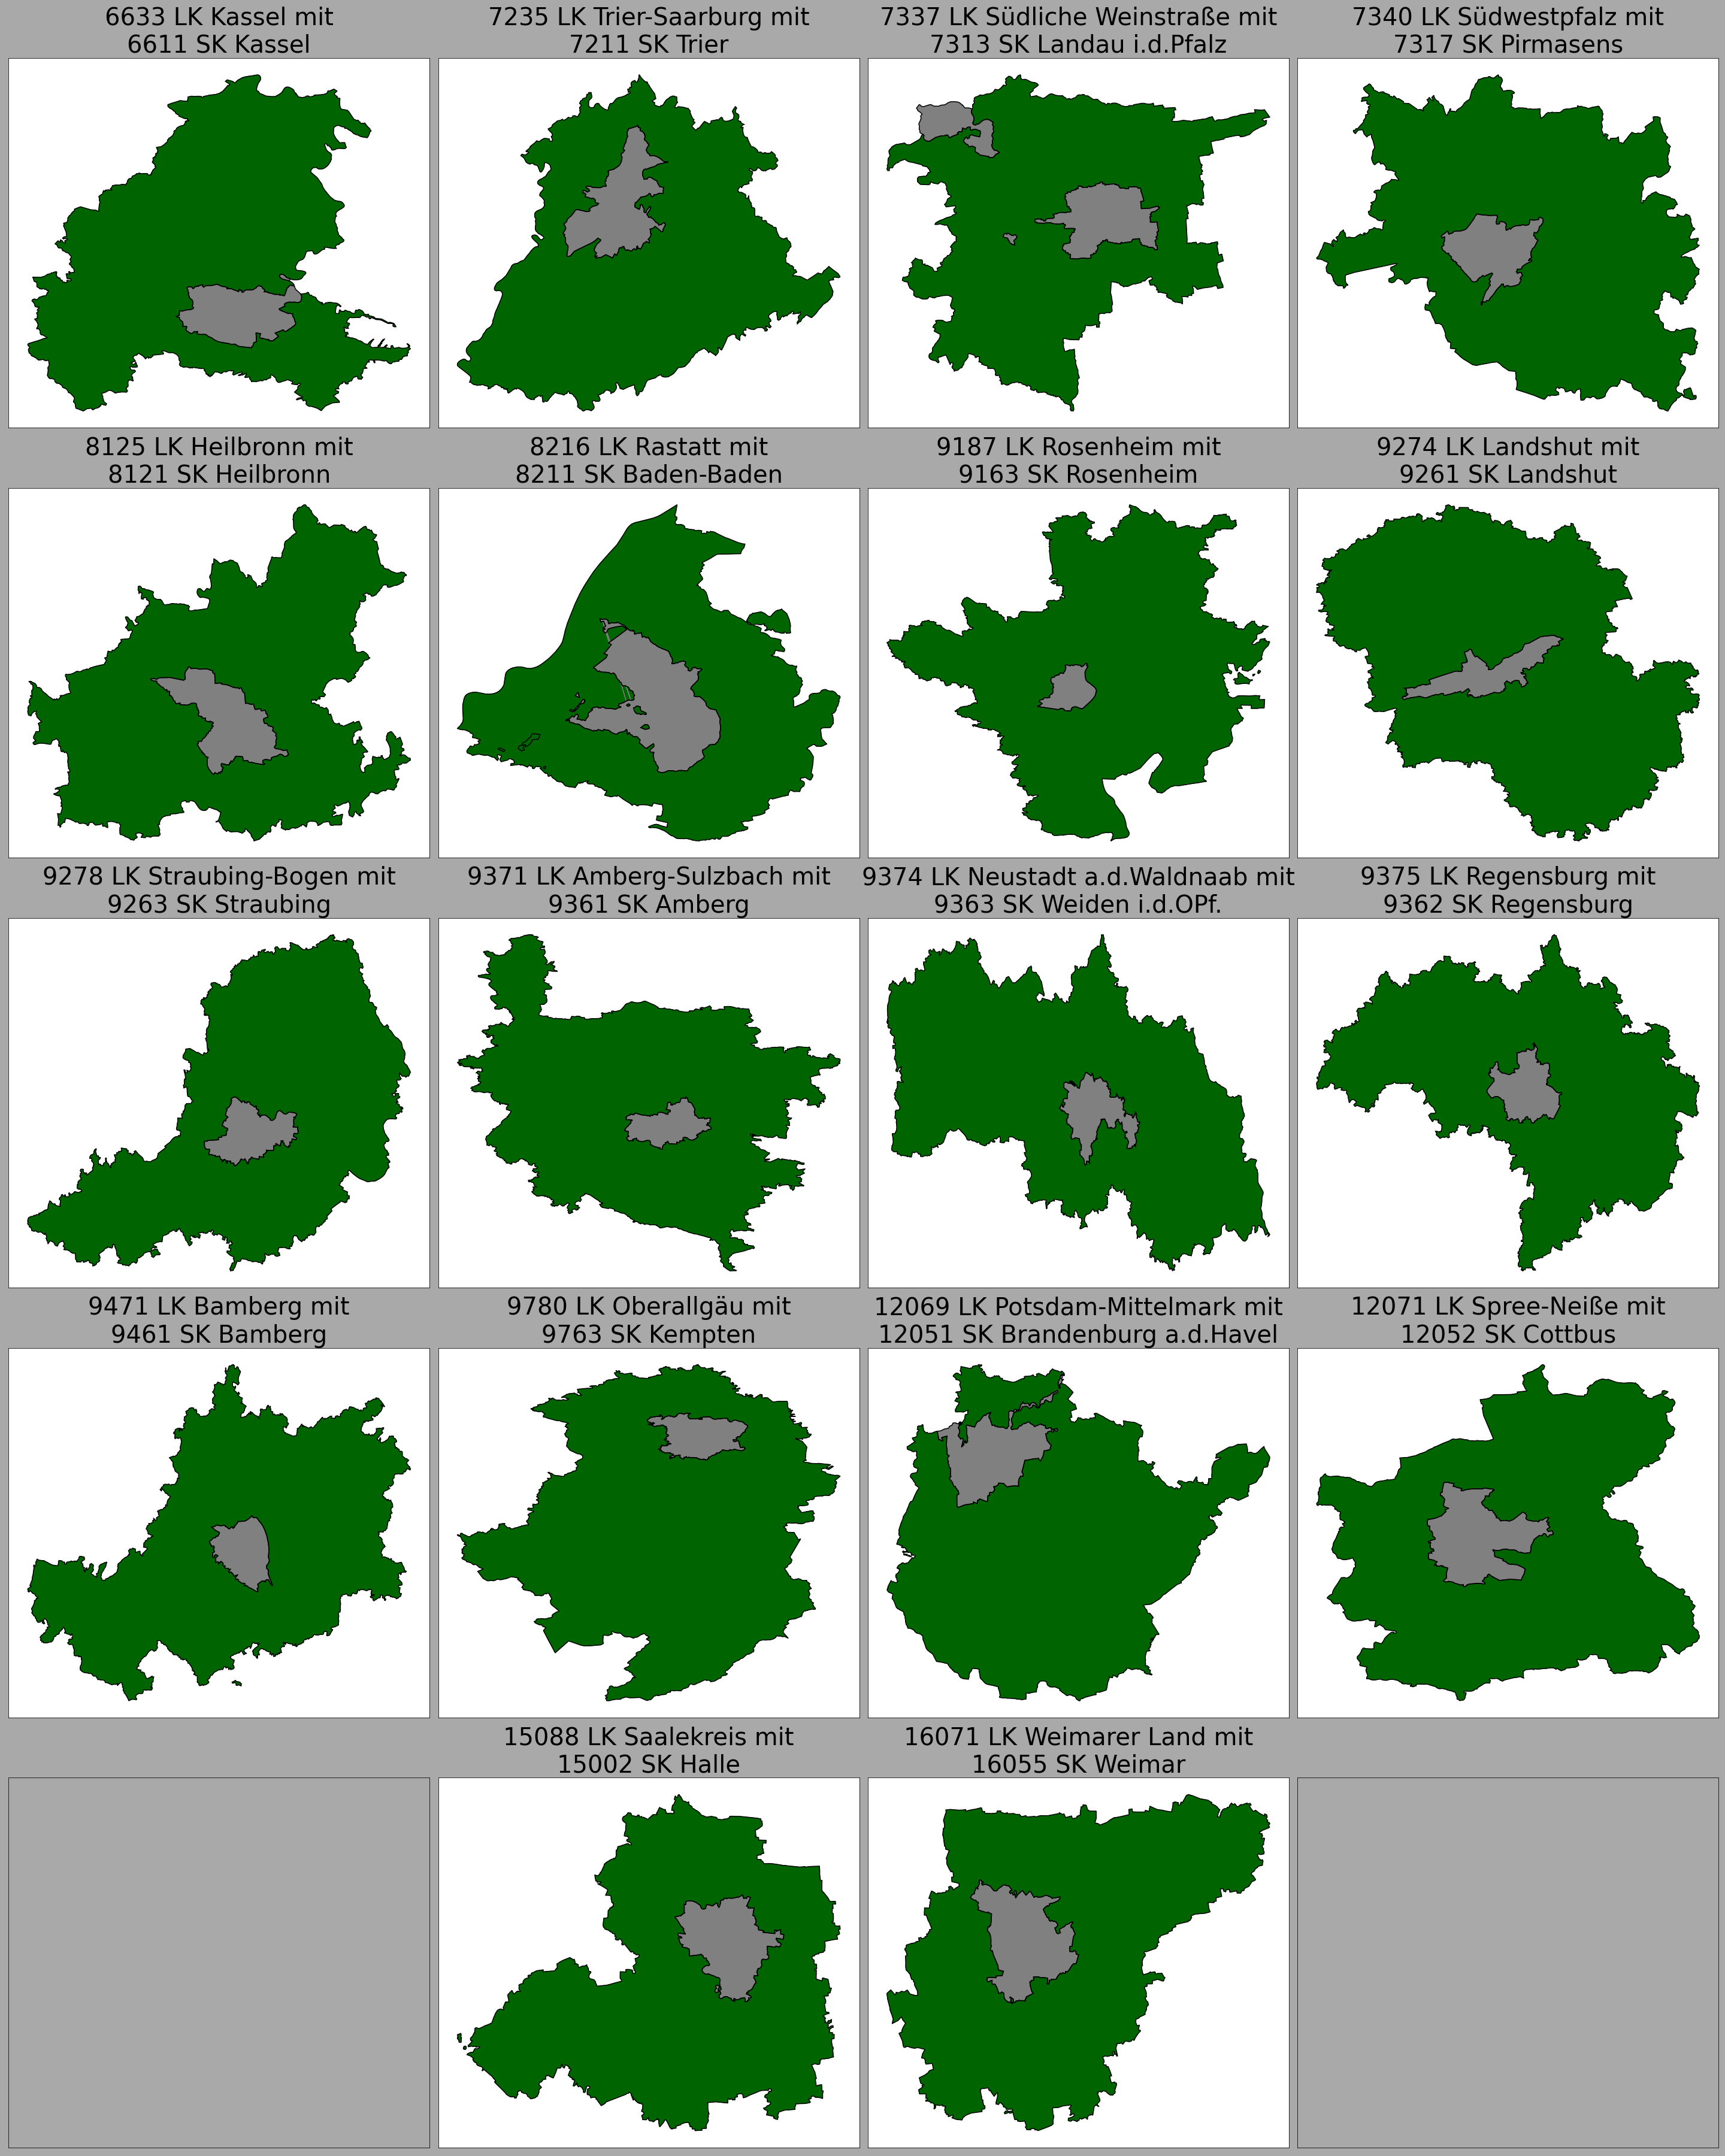
\includegraphics[width=\textwidth]{figures/Vorgehensweise/selected_counties.png}
    \caption{Die ausgewählten Landkreise mit den Stadtkreisen, die sie jeweils umgeben. In Grün jeweils der Landkreis und in Dunkelgrau der Stadtkreis, der umschlossen wird.}
    \label{fig:selected_counties}
\end{figure}
In dieser Arbeit werden nur Korrelationen mit einem zeitlichen Versatz zwischen $\tau=-50$ und $\tau=50$ betrachtet, da zum einen eine Interpretation für eine Verschiebung von mehr als 50 Tagen sehr schwierig ist und zum anderen einzelne Ausreißer bei größeren Verschiebungen stärker ins Gewicht fallen, weil immer weniger Produkte aufsummiert werden. Dies fällt auch in \autoref{fig:correlation_Flensburg_Kiel_scaled_autocorrelation} im Vergleich zu \autoref{fig:correlation_Flensburg_Kiel} an den Rändern der Graphen auf.

Um ein detailliertes Bild zu erhalten, werden zudem Korrelationsanalysen für die Verschiebungen $\tau\in[-30,30]$ und $\tau\in[-14,14]$ durchgeführt.

\subsection{Korrelation einzelner ausgewählter Städte und Landkreise}\label{sec:selected_counties}
Zum Einstieg werden die Korrelationen zwischen den Landkreisen aus \autoref{fig:selected_counties} und den Stadtkreisen, die sie umgeben, berechnet.
An ihnen lässt sich besonders gut testen, ob sich in den Korrelationswerten zwischen einer Stadt und ihrem Umland eine zeitliche Verschiebung feststellen lässt.
Um die festgestellten zeitlichen Verschiebungen einzuordnen, wird zudem ermittelt, bei wieviel Prozent der Korrelationen aller deutschen Landkreise untereinander der höchste Korrelationswert bei einer Verschiebung von $\tau = 0$ zu finden ist.

Für die ausgewählten Landkreis-Stadtkreis-Paare werden Korrelationsanalysen durchgeführt, wie in \autoref{sec:BeschreibungKorrelationsanalyse} beschrieben. Da es sich um eine übersichtliche Datenmenge handelt und für jedes Gebiet nur eine Korrelation geprüft wird, werden die Werte, welche normalerweise in Matrixform dargestellt werden, explizit ausgegeben.
\subsection{Korrelationsanalysen aller Landkreise und Regierungsbezirke}\label{sec:Vorgehensweise:Korrelationsanalysen aller Landkreise und Regierungsbezirke}

